% - Základní funkce a model spolupráce
%   - Repozitáře (veřejné / soukromé, forky)
%     - Fork: kopie repozitáře pod jiným uživatelem, smysl pro přispívání do cizích projektů
%     - Hvězdičky, watchers
%   - Issues
%     - Sledování chyb a požadavků na funkce
%     - Labely (kategorizace, prioritizace), milníky, přiřazení
%   - Pull Requesty (PR)
%     - Contribution workflow: fork → větev → commit → PR → review → merge
%     - Review proces: review komentáře, schvalování, požadované změny
%     - Labely na PR (stejný systém jako Issues)
%     - Draft PR, auto-merge
%     - Propojení PR s Issues (closing keywords: "Closes #123")
%   - GitHub Actions (CI/CD)
%     - Workflow soubory v .github/workflows/ (YAML)
%     - Triggery (push, PR, schedule, workflow_dispatch...)
%     - Runners (GitHub-hosted vs. self-hosted)
%     - Využití v kontextu monitoringu: automatické spouštění aktualizací dat
%   - Projekty a milníky (GitHub Projects)

\section{Základní funkce a model spolupráce}
\label{sec:github:zakladni_funkce_model_spoluprace}
V~této sekci jsou popsány nejpoužívanější funkce GitHubu a~modely interakce mezi vývojáři~\cite{github_docs}.

\subsection{Repozitáře}
\label{subsec:github:repozitare}
Repozitář představuje základní prvek na GitHubu. Jedná se o~místo, kde je ukládán zdrojový kód a~jiné soubory projektu. Repozitáře mohou být veřejné nebo soukromé a~mohou mít více spolupracovníků~\cite{github_docs}.

\subsubsection*{Forky}
\label{subsubsec:github:forky}
Fork je repozitář vytvořený pod jiným uživatelským účtem, který vychází z~původního repozitáře a~sdílí jeho historii. Forky jsou využívány primárně pro přispívání do cizích projektů. Nejčastěji je vytvořen fork, v~něm jsou provedeny změny a~následně je otevřen \PR do původního repozitáře. Možnost navrhnout sloučení změn do původního projektu je hlavním rozdílem mezi forkem a~klonem repozitáře. Fork se tedy částečně chová jako samostatná větev, avšak bez nutnosti mít přímý zápis do původního repozitáře. Tento způsob práce umožňuje bezpečně experimentovat bez přímého ovlivnění původního projektu~\cite{github_pull_requests_docs}.

Každý fork je plně samostatný a~má vlastní větve, členy, issues, pull requesty, wiki a~další funkce~\cite{github_docs}.

\subsection{Issues}
\label{subsec:github:issues}
Issues (neboli problémy) představují jednu ze základních a~nejvyužívanějších funkcí GitHubu. Jsou používány ke sledování chyb, nápadů, požadavků na funkce a~dalších úkolů spojených s~projektem~\cite{github_issues_docs}.

Jedna issue může mít sub-issues, aby mohl být větší úkol rozdělen na více menších částí. Pokud je issue závislá na dokončení jiné issue, lze tuto závislost explicitně vyjádřit a~označit úkol jako blokovaný. Současně mohou být přidávána metadata, například labely, typ issue, přiřazení nebo milníky. Issue může být přiřazena konkrétnímu uživateli, což usnadňuje organizaci práce i~sledování odpovědnosti~\cite{github_issues_docs}.

Labely představují klíčový nástroj pro kategorizaci a~prioritizaci nejen issues, ale také \PR a~diskuzí. Labely jsou vytvářeny v~rámci repozitáře a~následně přiřazovány jednotlivým issues, pull requestům a~diskuzím. V~ každém novém repozitáři je k~dispozici základní sada labelů, například \code{bug}, \code{enhancement}, \code{question} nebo \code{help wanted}. Tyto labely mohou být podle potřeby upravovány, přidávány i~odstraňovány~\cite{github_issues_docs}.

\subsubsection*{Pull Requests}
\label{subsubsec:github:pull_requests}
Pull requests (\PR{}) představují mechanismus, kterým může být navrženo začlenění změn do projektu. Umožňují vytvořit požadavek na provedení změn ve zdrojovém kódu. Následně může proběhnout kontrola změn a~diskuze nad konkrétními částmi kódu. Tím je podporováno udržení kvality kódu a~včasné odhalení chyb~\cite{github_pull_requests_docs}.

Typický workflow zahrnuje vytvoření forku a~založení nové větve, například pro konkrétní issue. Poté jsou provedeny změny a vytvořen \PR v rámci forku. Pokud je všechno vpořádku, je otevřen \PR v originálním repozitáři pro navržení začlenění změn.

\begin{figure}[h]
  \centering
  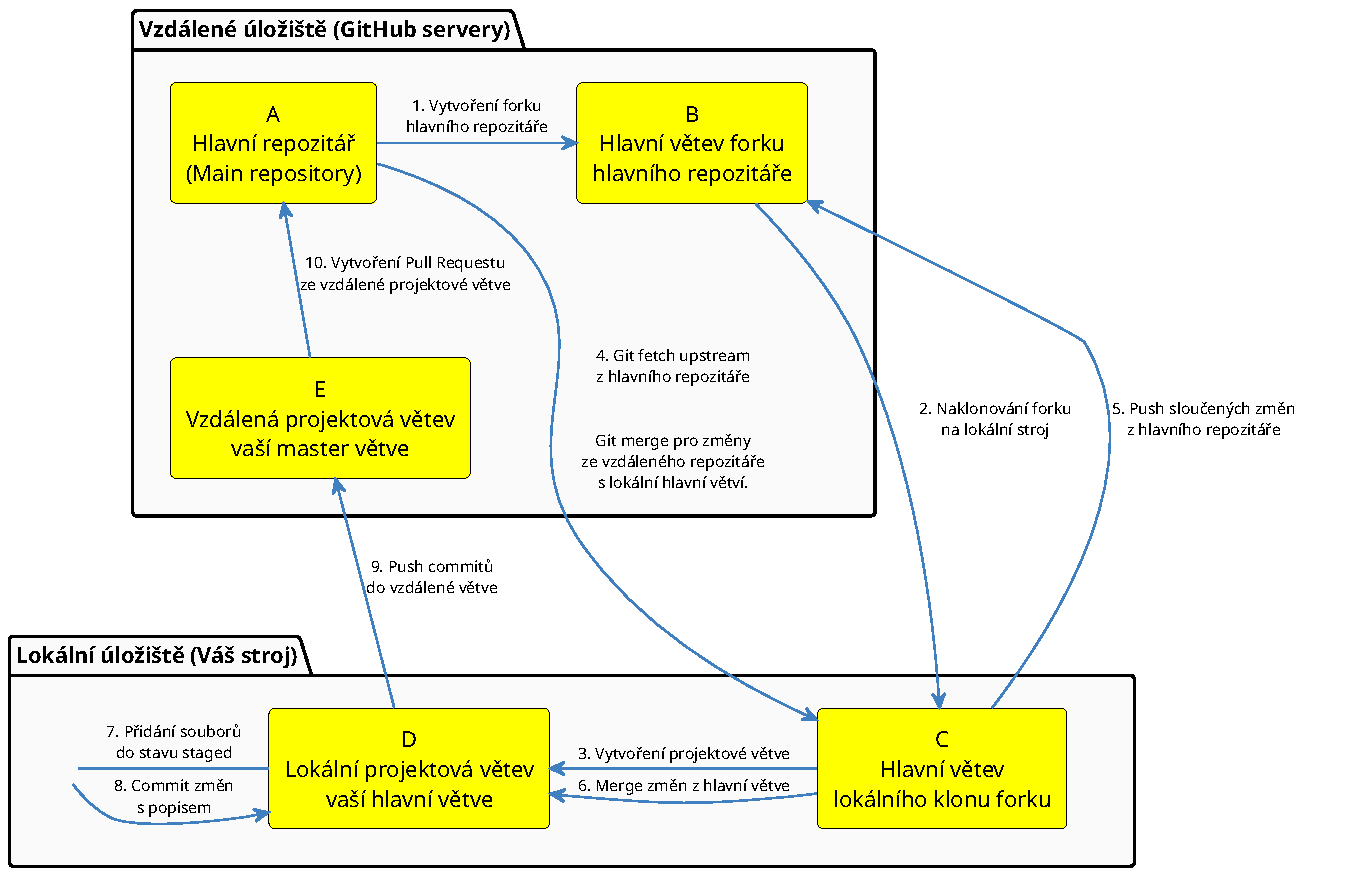
\includegraphics[width=\textwidth]{figures/github/fork-workflow.pdf}
  \caption{Průběh práce s forkem na GitHubu}
  \label{fig:github:fork-workflow}
\end{figure}
